 % arara: clean: { files: [thesis.aux, thesis.bbl, thesis.blg, thesis.dvi, thesis.fdb_latexmk, thesis.fls, thesis.idx, thesis.ilg, thesis.ind, thesis.lof, thesis.log, thesis.lot, thesis.nlo, thesis.nls, thesis.out, thesis.pdf, thesis.ps, thesis.toc]}
% arara: latex:  { shell: yes }
% arara: bibtex
% arara: nomencl
% arara: latex
% arara: makeindex
% arara: latex:  { shell: yes }
% arara: dvips
% arara: ps2pdf

% ******************************* PhD Thesis Template **************************
% Please have a look at the README.md file for info on how to use the template

\documentclass[a4paper,12pt,times,numbered,print,index]{Classes/PhDThesisPSnPDF}

% ******************************************************************************
% ******************************* Class Options ********************************
% *********************** See README for more details **************************
% ******************************************************************************

% `a4paper'(The University of Cambridge PhD thesis guidelines recommends a page
% size a4 - default option) or `a5paper': A5 Paper size is also allowed as per
% the Cambridge University Engineering Deparment guidelines for PhD thesis
%
% `11pt' or `12pt'(default): Font Size 10pt is NOT recommended by the University
% guidelines
%
% `oneside' or `twoside'(default): Printing double side (twoside) or single
% side.
%
% `print': Use `print' for print version with appropriate margins and page
% layout. Leaving the options field blank will activate Online version.
%
% `index': For index at the end of the thesis
%
% `draft': For draft mode without loading any images (same as draft in book)
%
% `abstract': To generate only the title page and abstract page with
% dissertation title and name, to submit to the Student Registry
%
% `chapter`: This option enables only the specified chapter and it's references
%  Useful for review and corrections.
%
% ************************* Custom Page Margins ********************************
%
% `custommargin`: Use `custommargin' in options to activate custom page margins,
% which can be defined in the preamble.tex. Custom margin will override
% print/online margin setup.
%
% *********************** Choosing the Fonts in Class Options ******************
%
% `times' : Times font with math support. (The Cambridge University guidelines
% recommend using times)
%
% `fourier': Utopia Font with Fourier Math font (Font has to be installed) 
%            It's a free font.
%
% `customfont': Use `customfont' option in the document class and load the
% package in the preamble.tex
%
% default or leave empty: `Latin Modern' font will be loaded.
%
% ********************** Choosing the Bibliography style ***********************
%
% `authoryear': For author-year citation eg., Krishna (2013)
%
% `numbered': (Default Option) For numbered and sorted citation e.g., [1,5,2]
%
% `custombib': Define your own bibliography style in the `preamble.tex' file.
%              `\RequirePackage[square, sort, numbers, authoryear]{natbib}'. 
%              This can be also used to load biblatex instead of natbib 
%              (See Preamble) 
%
% **************************** Choosing the Page Style *************************
%
% `default (leave empty)': For Page Numbers in Header (Left Even, Right Odd) and
% Chapter Name in Header (Right Even) and Section Name (Left Odd). Blank Footer.
%
% `PageStyleI': Chapter Name next & Page Number on Even Side (Left Even).
% Section Name & Page Number in Header on Odd Side (Right Odd). Footer is empty.
%
% `PageStyleII': Chapter Name on Even Side (Left Even) in Header. Section Number
% and Section Name in Header on Odd Side (Right Odd). Page numbering in footer


% ********************************** Preamble **********************************
% Preamble: Contains packages and user-defined commands and settings
%!TEX root = ../thesis.tex
% !TEX TS-program = xelatex
% ****************************** Misc ******************************************
\usepackage{blindtext}
% ******************************************************************************
% ****************************** Custom Margin *********************************
% Add `custommargin' in the document class options to use this section
% Set {innerside margin / outerside margin / topmargin / bottom margin}  and
% other page dimensions
\ifsetCustomMargin
  \RequirePackage[left=37mm,right=30mm,top=35mm,bottom=30mm]{geometry}
  \setFancyHdr % To apply fancy header after geometry package is loaded
\fi

% Add spaces between paragraphs
%\setlength{\parskip}{0.5em}
% Ragged bottom avoids extra whitespaces between paragraphs
\raggedbottom
% To remove the excess top spacing for enumeration, list and description
%\usepackage{enumitem}
%\setlist[enumerate,itemize,description]{topsep=0em}

% *****************************************************************************
% ******************* Fonts (like different typewriter fonts etc.)*************
\usepackage{ wasysym }

% Add `customfont' in the document class option to use this section

\ifsetCustomFont
  % Set your custom font here and use `customfont' in options. Leave empty to
  % load computer modern font (default LaTeX font).
  \RequirePackage{mathpazo}
  \usepackage{amsmath}
  \usepackage{newpxtext}
  %\usepackage{mathpazo}
  %\usepackage[T1]{fontenc}
  %\usepackage{fontspec}

  \usepackage{sectsty}
  \usepackage{roboto}
  \allsectionsfont{\sffamily} % <---- omitting \bfseries still gives bold font
  %\usepackage{xfrac,fontspec,unicode-math}
  %\setmathfont[version=lm]{Latin Modern Math}
  % For use with XeLaTeX
  %  \setmainfont[
  %    Path              = ./libertine/opentype/,
  %    Extension         = .otf,
  %    UprightFont = LinLibertine_R,
  %    BoldFont = LinLibertine_RZ, % Linux Libertine O Regular Semibold
  %    ItalicFont = LinLibertine_RI,
  %    BoldItalicFont = LinLibertine_RZI, % Linux Libertine O Regular Semibold Italic
  %  ]
  %  {libertine}
  %  % load font from system font
  %  \newfontfamily\libertinesystemfont{Linux Libertine O}
\fi

% *****************************************************************************
% **************************** Custom Packages ********************************

% ************************* Algorithms and Pseudocode **************************

\usepackage{algpseudocode}


% ********************Captions and Hyperreferencing / URL **********************

% Captions: This makes captions of figures use a boldfaced small font.
%\RequirePackage[small,bf]{caption}

\RequirePackage[labelsep=space,tableposition=top,small,bf]{caption}
\renewcommand{\figurename}{Fig.} %to support older versions of captions.sty


% *************************** Graphics and figures *****************************

%\usepackage{rotating}
%\usepackage{wrapfig}

% Uncomment the following two lines to force Latex to place the figure.
% Use [H] when including graphics. Note 'H' instead of 'h'
%\usepackage{float}
%\restylefloat{figure}

% Subcaption package is also available in the sty folder you can use that by
% uncommenting the following line
% This is for people stuck with older versions of texlive
%\usepackage{sty/caption/subcaption}
\usepackage{subcaption}

% ********************************** Tables ************************************
\usepackage{booktabs} % For professional looking tables
\usepackage{multirow}

\usepackage{multicol}
\usepackage{longtable}
\usepackage{tabularx}


% *********************************** SI Units *********************************
\usepackage[allow-number-unit-breaks=true,separate-uncertainty=true,multi-part-units=single,binary-units=true]{siunitx} % use this package module for SI units

% ******************************* Line Spacing *********************************

% Choose linespacing as appropriate. Default is one-half line spacing as per the
% University guidelines

% \doublespacing
 \onehalfspacing
% \singlespacing

\usepackage{enumitem}

% ************************ Formatting / Footnote *******************************

% Don't break enumeration (etc.) across pages in an ugly manner (default 10000)
%\clubpenalty=500
%\widowpenalty=500

%\usepackage[perpage]{footmisc} %Range of footnote options


% *****************************************************************************
% *************************** Bibliography  and References ********************

%\usepackage{cleveref} %Referencing without need to explicitly state fig /table

% Add `custombib' in the document class option to use this section
% \ifuseCustomBib
   % \RequirePackage[numbers,sort&compress]{natbib} % CustomBib

% If you would like to use biblatex for your reference management, as opposed to the default `natbibpackage` pass the option `custombib` in the document class. Comment out the previous line to make sure you don't load the natbib package. Uncomment the following lines and specify the location of references.bib file


\RequirePackage[style=nature,date=year,backend=bibtex,doi=false,isbn=false,url=false,sorting=none,sortcites=true,doi=false,url=false,hyperref]{biblatex}
\addbibresource{./References/references.bib,./References/references.bib} %Location of references.bib only for biblatex, Do not omit the .bib extension from the filename.
\bibliography{References/references,References/_references} %Location of references.bib only for biblatex

% \fi

% changes the default name `Bibliography` -> `References'
\renewcommand{\bibname}{References}


% ******************************************************************************
% ************************* User Defined Commands ******************************
% ******************************************************************************

% *********** To change the name of Table of Contents / LOF and LOT ************

%\renewcommand{\contentsname}{My Table of Contents}
%\renewcommand{\listfigurename}{My List of Figures}
%\renewcommand{\listtablename}{My List of Tables}


% ********************** TOC depth and numbering depth *************************

\setcounter{secnumdepth}{2}
\setcounter{tocdepth}{2}


% ******************************* Nomenclature *********************************

% To change the name of the Nomenclature section, uncomment the following line

%\renewcommand{\nomname}{Symbols}


% ********************************* Appendix ***********************************

% The default value of both \appendixtocname and \appendixpagename is `Appendices'. These names can all be changed via:

%\renewcommand{\appendixtocname}{List of appendices}
%\renewcommand{\appendixname}{Appndx}

% *********************** Configure Draft Mode **********************************

% Uncomment to disable figures in `draft'
%\setkeys{Gin}{draft=true}  % set draft to false to enable figures in `draft'

% These options are active only during the draft mode
% Default text is "Draft"
%\SetDraftText{DRAFT}

% Default Watermark location is top. Location (top/bottom)
%\SetDraftWMPosition{bottom}

% Draft Version - default is v1.0
%\SetDraftVersion{v1.1}

% Draft Text grayscale value (should be between 0-black and 1-white)
% Default value is 0.75
%\SetDraftGrayScale{0.8}


% ******************************** Todo Notes **********************************
%% Uncomment the following lines to have todonotes.

\ifsetDraft
	\usepackage[colorinlistoftodos]{todonotes}
	\newcommand{\mynote}[1]{\todo[author=ctr26,size=\small,inline,color=green!40]{#1}}
\else
	\newcommand{\mynote}[1]{}
	\newcommand{\listoftodos}{}
\fi

% Example todo: \mynote{Hey! I have a note}

%%%
\usepackage{pgfplots}
\usepackage{tikzscale}
\usepackage{helvet}

\usepackage[eulergreek]{sansmath}
\pgfplotsset{
  tick label style = {font=\sansmath\sffamily\footnotesize},
  %every axis label = {font=\sansmath\sffamily},
  %legend style = {font=\sansmath\sffamily},
  %label style = {font=\sansmath\sffamily}
}
\usepackage{roboto}
% https://github.com/matlab2tikz/matlab2tikz/issues/672
\newlength{\figwidth}
\newlength{\figheight}

\setlength{\figwidth}{0.4\textwidth}
\setlength{\figheight}{0.6180\figwidth}


\usepackage{graphicx}
\usepackage{xcolor}
\definecolor{darkblue}{rgb}{0,0,0.5}
\usepackage{transparent}

\usepackage{import}

\usepackage{pdflscape}

\usepackage{dpfloat}
\usepackage{multicol}

\usepackage{mhchem}
\usepackage{wrapfig}
\usepackage[super]{nth}


\newcommand{\nosection}[1]{%
  \refstepcounter{section}%
  \addcontentsline{toc}{section}{\protect\numberline{\thesection}#1}%
  \markright{#1}}


  \usepackage{tikz}
  \usepackage{graphicx}
  \usetikzlibrary{positioning}


% ************************ Thesis Information & Meta-data **********************
% Thesis title and author information, refernce file for biblatex
% ************************ Thesis Information & Meta-data **********************
%% The title of the thesis
\title{Writing your PhD thesis in \texorpdfstring{\\ \LaTeX2e}{LaTeX2e}}
%\texorpdfstring is used for PDF metadata. Usage:
%\texorpdfstring{LaTeX_Version}{PDF Version (non-latex)} eg.,
%\texorpdfstring{$sigma$}{sigma}

%% Subtitle (Optional)
\subtitle{Using the CUED template}

%% The full name of the author
\author{Krishna Kumar}

%% Department (eg. Department of Engineering, Maths, Physics)
\dept{Department of Engineering}

%% University and Crest
\university{University of Cambridge}
% Crest minimum should be 30mm.
%\crest{
\includegraphics[width=0.2\textwidth]{University_Crest}}
%% Use this crest, if you are using the college crest
%% Crest long miminum should be 65mm
\crest{
\includegraphics[width=0.45\textwidth]{University_Crest_Long}}

%% College shield [optional] 
% Crest minimum should be 30mm.
\collegeshield{
\includegraphics[width=0.2\textwidth]{CollegeShields/Kings}}

%% You can redefine the submission text:
% Default as per the University guidelines:
% ``This dissertation is submitted for the degree of''
%\renewcommand{\submissiontext}{change the default text here if needed}

%% Full title of the Degree
\degreetitle{Doctor of Philosophy}

%% College affiliation (optional)
\college{King's College}

%% Submission date
% Default is set as {\monthname[\the\month]\space\the\year}
%\degreedate{September 2014} 

%% Meta information
\subject{LaTeX} \keywords{{LaTeX} {PhD Thesis} {Engineering} {University of
Cambridge}}


% ***************************** Abstract Separate ****************************** 
% To printout only the titlepage and the abstract with the PhD title and the 
% author name for submission to the Student Registry, use the `abstract' option in
% the document class. 

\ifdefineAbstract
 \pagestyle{empty}
 \includeonly{Declaration/declaration, Abstract/abstract} 
\fi

% ***************************** Chapter Mode ***********************************
% The chapter mode allows user to only print particular chapters with references
% Title, Contents, Frontmatter are disabled by default
% Useful option to review a particular chapter or to send it to supervisior.
% To use choose `chapter' option in the document class

\ifdefineChapter
 \includeonly{Chapter3/chapter3} 
\fi

% ******************************** Front Matter ********************************
\begin{document}

\frontmatter

\begin{titlepage}

\maketitle

\end{titlepage}

%!TEX root = ../thesis.tex
% ******************************* Thesis Dedidcation ********************************

\begin{dedication}

% I would like to dedicate this thesis to booze

\end{dedication}

% Thesis Declaration ---------------------------------------------------

\begin{declaration} %this creates the heading for the dedication page

I hereby declare that except where specific reference is made to the work of others, the contents of this dissertation are original and have not been submitted in whole or in part for consideration for any other degree or qualification in this, or any other University. This dissertation is entirely the result of my own work and includes nothing which is the outcome of work done in collaboration, except where specified in the text. This dissertation contains less than 65,000 words, excluding table of contents, tables, figures, titles, footnotes, references and appendices and 150 figures.

%Permission has been granted by board of graduate studies to exceed the recommended limits 150 figures and to include a CD-ROM in the dissertation. This dissertation is presented less than 65,000 words and 210 figures.
\flushright

Krishna Kumar\\
2013
\end{declaration}


% ************************** Thesis Acknowledgements **************************

\begin{acknowledgements}
\begin{description}% I would like to dedicate this thesis to booze
  \item \emph{Dr.~Eric Rees} for his compassion and brilliance.
  \item \emph{Dale}, \emph{Jean}, \emph{Phil}, \emph{Jimmy}, \emph{Jonny} and \emph{Wag} for being my anchors
  \item \emph{Roxine Staats} for her tireless editing and support
  \item \emph{Dr.~Nathan Curry} for guiding me for 5 years
  \item \emph{Dr.~Chris Rowlands} for his hours of effort, his patience, his creativity and his wealth of knowledge
  \item \emph{Pedro Vallejo} for his boundless care and consideration
  \item \emph{James Manton} for his ever-sagely scientific opinion
  \item \emph{Madeleine Eve Rodgers} for showing me how to work with people
  \item \emph{Dr.~Colin Hockings} for his infinite patience with my minimal knowledge of biology
  \item \emph{Dr.~Romain Laine} for his enthusiasm and wisdom
  \item \emph{Dr.~Aleks Chjemieklvia} for his time and supervision
  \item \emph{Dr.~Florian Strohl} for his exquisite knowledge of optics
  \item \emph{Dr.~Laurie Young} for his mentorship and advice
  % \item \emph{Victoire Cachoux} for being a dear friend at a trying time
  \item \emph{Magdalene College} for providing me a home, a family, friends and support
  \item \emph{Magdalene Boat Club} for helping me grow
  \item \emph{St Edmunds College} for not turning me away
\end{description}
\end{acknowledgements}


% Thesis Abstract -----------------------------------------------------


%\begin{abstractslong}    %uncommenting this line, gives a different abstract heading
\begin{abstracts}        %this creates the heading for the abstract page

This is where you write your abstract ...


\end{abstracts}
%\end{abstractlongs}


% ----------------------------------------------------------------------


%%% Local Variables: 
%%% mode: latex
%%% TeX-master: "../thesis"
%%% End: 


% *********************** Adding TOC and List of Figures ***********************

\tableofcontents

\listoffigures

\listoftables 

% \printnomenclature[space] space can be set as 2.5cm between symbol and
% description
\printnomencl

% ******************************** Main Matter *********************************
\mainmatter

%*****************************************************************************************
%*********************************** First Chapter ***************************************
%*****************************************************************************************

\chapter{Getting Started}  %Title of the First Chapter

\ifpdf
    \graphicspath{{Chapter1/Figs/Raster/}{Chapter1/Figs/PDF/}{Chapter1/Figs/}}
\else
    \graphicspath{{Chapter1/Figs/Vector/}{Chapter1/Figs/}}
\fi


%********************************** %First Section  **************************************
\section{What is Loren Ipsum? Title with Math \texorpdfstring{$\sigma$}{[sigma]}} %Section - 1.1 

Lorem Ipsum is simply dummy text of the printing and typesetting industry (see Section~\ref{section1.3}). Lorem Ipsum~\citep{Aup91} has been the industry's standard dummy text ever since the 1500s, when an unknown printer took a galley of type and scrambled it to make a type specimen book. It has survived not only five centuries, but also the leap into electronic typesetting, remaining essentially unchanged. It was popularised in the 1960s with the release of Letraset sheets containing Lorem Ipsum passages, and more recently with desktop publishing software like Aldus PageMaker including versions of Lorem Ipsum~\citep{AAB95,Con90,LM65}.

The most famous equation in the world: $E^2 = (m_0c^2)^2 + (pc)^2$, which is known as the \textbf{energy-mass-momentum} relation as an in-line equation.

A {\em \LaTeX{} class file}\index{\LaTeX{} class file@LaTeX class file} is a file, which holds style information for a particular \LaTeX{}.

\begin{eqnarray}
CIF: \hspace*{5mm}F_0^j(a) &=& \frac{1}{2\pi \iota} \oint_{\gamma} \frac{F_0^j(z)}{z - a} dz
\end{eqnarray}

\nomenclature[z-cif]{$CIF$}{Cauchy's Integral Formula}                                % first letter Z is for Acronyms 
\nomenclature[a-F]{$F$}{complex function}                                                   % first letter A is for Roman symbols
\nomenclature[g-p]{$\pi$}{ $\simeq 3.14\ldots$}                                             % first letter G is for Greek Symbols
\nomenclature[g-i]{$\iota$}{unit imaginary number $\sqrt{-1}$}                      % first letter G is for Greek Symbols
\nomenclature[g-g]{$\gamma$}{a simply closed curve on a complex plane}  % first letter G is for Greek Symbols
\nomenclature[x-i]{$\oint_\gamma$}{integration around a curve $\gamma$} % first letter X is for Other Symbols
\nomenclature[r-j]{$j$}{superscript index}                                                       % first letter R is for superscripts
\nomenclature[s-0]{$0$}{subscript index}                                                        % first letter S is for subscripts


%********************************** %Second Section  *************************************
\section{Why do we use Loren Ipsum?} %Section - 1.2


It is a long established fact that a reader will be distracted by the readable content of a page when looking at its layout. The point of using Lorem Ipsum is that it has a more-or-less normal distribution of letters, as opposed to using `Content here, content here', making it look like readable English. Many desktop publishing packages and web page editors now use Lorem Ipsum as their default model text, and a search for `lorem ipsum' will uncover many web sites still in their infancy. Various versions have evolved over the years, sometimes by accident, sometimes on purpose (injected humour and the like).

%********************************** % Third Section  *************************************
\section{Where does it come from?}  %Section - 1.3 
\label{section1.3}

Contrary to popular belief, Lorem Ipsum is not simply random text. It has roots in a piece of classical Latin literature from 45 BC, making it over 2000 years old. Richard McClintock, a Latin professor at Hampden-Sydney College in Virginia, looked up one of the more obscure Latin words, consectetur, from a Lorem Ipsum passage, and going through the cites of the word in classical literature, discovered the undoubtable source. Lorem Ipsum comes from sections 1.10.32 and 1.10.33 of "de Finibus Bonorum et Malorum" (The Extremes of Good and Evil) by Cicero, written in 45 BC. This book is a treatise on the theory of ethics, very popular during the Renaissance. The first line of Lorem Ipsum, "Lorem ipsum dolor sit amet..", comes from a line in section 1.10.32.

The standard chunk of Lorem Ipsum used since the 1500s is reproduced below for those interested. Sections 1.10.32 and 1.10.33 from ``de Finibus Bonorum et Malorum" by Cicero are also reproduced in their exact original form, accompanied by English versions from the 1914 translation by H. Rackham

``Lorem ipsum dolor sit amet, consectetur adipisicing elit, sed do eiusmod tempor incididunt ut labore et dolore magna aliqua. Ut enim ad minim veniam, quis nostrud exercitation ullamco laboris nisi ut aliquip ex ea commodo consequat. Duis aute irure dolor in reprehenderit in voluptate velit esse cillum dolore eu fugiat nulla pariatur. Excepteur sint occaecat cupidatat non proident, sunt in culpa qui officia deserunt mollit anim id est laborum."

Section 1.10.32 of ``de Finibus Bonorum et Malorum", written by Cicero in 45 BC: ``Sed ut perspiciatis unde omnis iste natus error sit voluptatem accusantium doloremque laudantium, totam rem aperiam, eaque ipsa quae ab illo inventore veritatis et quasi architecto beatae vitae dicta sunt explicabo. Nemo enim ipsam voluptatem quia voluptas sit aspernatur aut odit aut fugit, sed quia consequuntur magni dolores eos qui ratione voluptatem sequi nesciunt. Neque porro quisquam est, qui dolorem ipsum quia dolor sit amet, consectetur, adipisci velit, sed quia non numquam eius modi tempora incidunt ut labore et dolore magnam aliquam quaerat voluptatem. Ut enim ad minima veniam, quis nostrum exercitationem ullam corporis suscipit laboriosam, nisi ut aliquid ex ea commodi consequatur? Quis autem vel eum iure reprehenderit qui in ea voluptate velit esse quam nihil molestiae consequatur, vel illum qui dolorem eum fugiat quo voluptas nulla pariatur?"

1914 translation by H. Rackham: ``But I must explain to you how all this mistaken idea of denouncing pleasure and praising pain was born and I will give you a complete account of the system, and expound the actual teachings of the great explorer of the truth, the master-builder of human happiness. No one rejects, dislikes, or avoids pleasure itself, because it is pleasure, but because those who do not know how to pursue pleasure rationally encounter consequences that are extremely painful. Nor again is there anyone who loves or pursues or desires to obtain pain of itself, because it is pain, but because occasionally circumstances occur in which toil and pain can procure him some great pleasure. To take a trivial example, which of us ever undertakes laborious physical exercise, except to obtain some advantage from it? But who has any right to find fault with a man who chooses to enjoy a pleasure that has no annoying consequences, or one who avoids a pain that produces no resultant pleasure?"

Section 1.10.33 of ``de Finibus Bonorum et Malorum", written by Cicero in 45 BC: ``At vero eos et accusamus et iusto odio dignissimos ducimus qui blanditiis praesentium voluptatum deleniti atque corrupti quos dolores et quas molestias excepturi sint occaecati cupiditate non provident, similique sunt in culpa qui officia deserunt mollitia animi, id est laborum et dolorum fuga. Et harum quidem rerum facilis est et expedita distinctio. Nam libero tempore, cum soluta nobis est eligendi optio cumque nihil impedit quo minus id quod maxime placeat facere possimus, omnis voluptas assumenda est, omnis dolor repellendus. Temporibus autem quibusdam et aut officiis debitis aut rerum necessitatibus saepe eveniet ut et voluptates repudiandae sint et molestiae non recusandae. Itaque earum rerum hic tenetur a sapiente delectus, ut aut reiciendis voluptatibus maiores alias consequatur aut perferendis doloribus asperiores repellat."

1914 translation by H. Rackham: ``On the other hand, we denounce with righteous indignation and dislike men who are so beguiled and demoralized by the charms of pleasure of the moment, so blinded by desire, that they cannot foresee the pain and trouble that are bound to ensue; and equal blame belongs to those who fail in their duty through weakness of will, which is the same as saying through shrinking from toil and pain. These cases are perfectly simple and easy to distinguish. In a free hour, when our power of choice is untrammelled and when nothing prevents our being able to do what we like best, every pleasure is to be welcomed and every pain avoided. But in certain circumstances and owing to the claims of duty or the obligations of business it will frequently occur that pleasures have to be repudiated and annoyances accepted. The wise man therefore always holds in these matters to this principle of selection: he rejects pleasures to secure other greater pleasures, or else he endures pains to avoid worse pains."

%*****************************************************************************************
%*********************************** Second Chapter **************************************
%*****************************************************************************************

\chapter{My Second Chapter}

\ifpdf
    \graphicspath{{Chapter2/Figs/Raster/}{Chapter2/Figs/PDF/}{Chapter2/Figs/}}
\else
    \graphicspath{{Chapter2/Figs/Vector/}{Chapter2/Figs/}}
\fi


\section[Short title]{Reasonably Long Section Title}

% Uncomment this line, when you have siunitx package loaded.
%The SI Units for dynamic viscosity is \si{\newton\second\per\metre\squared}.
I'm going to randomly include a picture Figure~\ref{fig:minion}.


If you have trouble viewing this document contact Krishna at: \href{mailto:kks32@cam.ac.uk}{kks32@cam.ac.uk} or raise an issue at \url{https://github.com/kks32/phd-thesis-template/}


\begin{figure}[htbp!] 
\centering    

\includegraphics[width=1.0\textwidth]{minion}
\caption[Minion]{This is just a long figure caption for the minion in Despicable Me from Pixar}
\label{fig:minion}
\end{figure}


\section*{Enumeration}
\begin{enumerate}
\item The first topic is dull
\item The second topic is duller
\begin{enumerate}
\item The first subtopic is silly
\item The second subtopic is stupid
\end{enumerate}
\item The third topic is the dullest
\end{enumerate}

\section*{itemize}
\begin{itemize}
\item The first topic is dull
\item The second topic is duller
\begin{itemize}
\item The first subtopic is silly
\item The second subtopic is stupid
\end{itemize}
\item The third topic is the dullest
\end{itemize}

\section*{description}
\begin{description}
\item[The first topic] is dull
\item[The second topic] is duller
\begin{description}
\item[The first subtopic] is silly
\item[The second subtopic] is stupid
\end{description}
\item[The third topic] is the dullest
\end{description}


\clearpage

\tochide\section{Hidden Section}
\textbf{Lorem ipsum dolor sit amet}, \textit{consectetur adipiscing elit}. In magna nisi, aliquam id blandit id, congue ac est. Fusce porta consequat leo. Proin feugiat at felis vel consectetur. Ut tempus ipsum sit amet congue posuere. Nulla varius rutrum quam. Donec sed purus luctus, faucibus velit id, ultrices sapien. Cras diam purus, tincidunt eget tristique ut, egestas quis nulla. Curabitur vel iaculis lectus. Nunc nulla urna, ultrices et eleifend in, accumsan ut erat. In ut ante leo. Aenean a lacinia nisl, sit amet ullamcorper dolor. Maecenas blandit, tortor ut scelerisque congue, velit diam volutpat metus, sed vestibulum eros justo ut nulla. Etiam nec ipsum non enim luctus porta in in massa. Cras arcu urna, malesuada ut tellus ut, pellentesque mollis risus.Morbi vel tortor imperdiet arcu auctor mattis sit amet eu nisi. Nulla gravida urna vel nisl egestas varius. Aliquam posuere ante quis malesuada dignissim. Mauris ultrices tristique eros, a dignissim nisl iaculis nec. Praesent dapibus tincidunt mauris nec tempor. Curabitur et consequat nisi. Quisque viverra egestas risus, ut sodales enim blandit at. Mauris quis odio nulla. Cras euismod turpis magna, in facilisis diam congue non. Mauris faucibus nisl a orci dictum, et tempus mi cursus.

Etiam elementum tristique lacus, sit amet eleifend nibh eleifend sed \footnote{My footnote goes blah blah blah! \dots}. Maecenas dapibu augue ut urna malesuada, non tempor nibh mollis. Donec sed sem sollicitudin, convallis velit aliquam, tincidunt diam. In eu venenatis lorem. Aliquam non augue porttitor tellus faucibus porta et nec ante. Proin sodales, libero vitae commodo sodales, dolor nisi cursus magna, non tincidunt ipsum nibh eget purus. Nam rutrum tincidunt arcu, tincidunt vulputate mi sagittis id. Proin et nisi nec orci tincidunt auctor et porta elit. Praesent eu dolor ac magna cursus euismod. Integer non dictum nunc.


\begin{landscape}

\section*{Subplots}
I can cite Wall-E (see Fig.~\ref{fig:WallE}) and Minions in despicable me (Fig.~\ref{fig:Minnion}) or I can cite the whole figure as Fig.~\ref{fig:animations}


\begin{figure}
  \centering
  \begin{subfigure}[b]{0.3\textwidth}
    
\includegraphics[width=\textwidth]{TomandJerry}
    \caption{Tom and Jerry}
    \label{fig:TomJerry}   
  \end{subfigure}             
  \begin{subfigure}[b]{0.3\textwidth}
    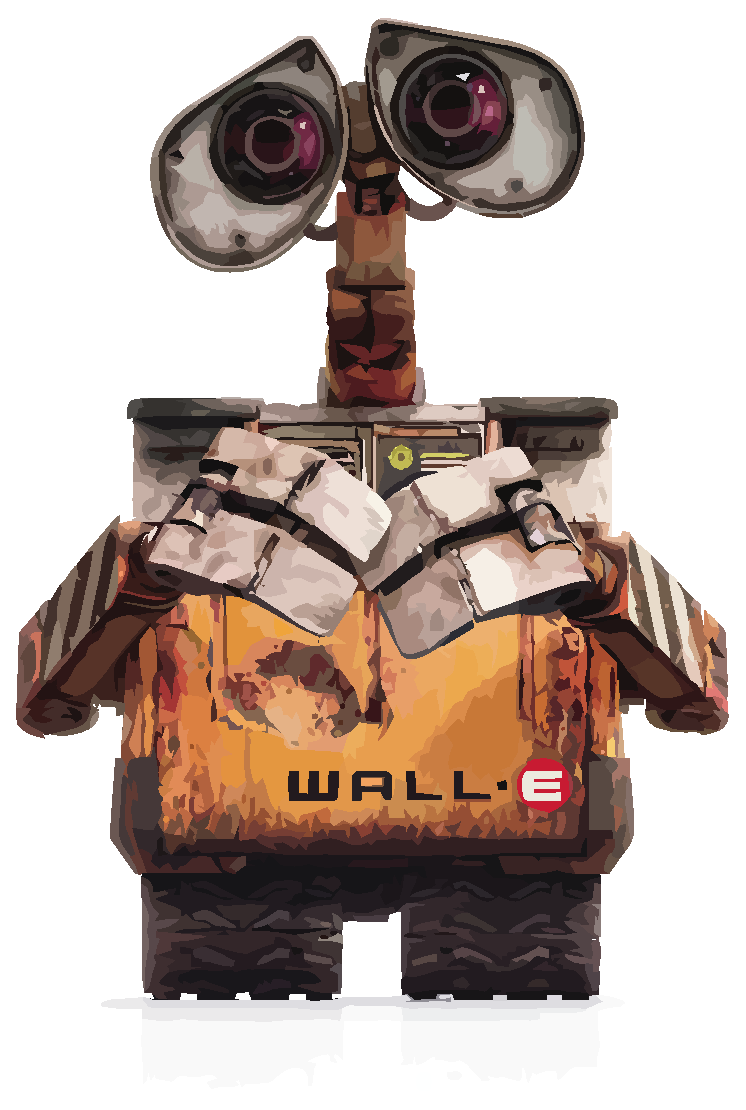
\includegraphics[width=\textwidth]{WallE}
    \caption{Wall-E}
    \label{fig:WallE}
  \end{subfigure}             
  \begin{subfigure}[b]{0.3\textwidth}
    
\includegraphics[width=\textwidth]{minion}
    \caption{Minions}
    \label{fig:Minnion}
  \end{subfigure}
  \caption{Best Animations}
  \label{fig:animations}
\end{figure}


\end{landscape}

%!TEX root = ../thesis.tex
%!TEX enableSynctex = true
%*******************************************************************************
%****************************** Third Chapter **********************************
%*******************************************************************************
% **************************** Define Graphics Path **************************
\ifpdf
    \graphicspath{{Chapter3/Figs/Raster/}{Chapter3/Figs/PDF/}{Chapter3/Figs/}}
\else
    \graphicspath{{Chapter3/Figs/Vector/}{Chapter3/Figs/}}
\fi

\chapter[Light-sheet microscopy combined with remote force measurements]{Light-sheet microscopy combined with remote force measurements}%:\\ \Large Correlating real-time viscoelastic changes with embryonic development}

%From Julien:
How multicellular organisms enact the morphogenetic programmes that ensure their characteristic forms remains an enigma. Genetic screens have yielded an array of essential structural, patterning and signalling pathways with which morphogenesis is orchestrated.
However, morphogenesis is ultimately a physical phenomenon that requires a physical explanation.  In vivo imaging of morphogenesis allows measurements that reveal stereotypical patterns in the cellular behaviour by individual and groups of cells.
These are indicative of active force generation but are insufficient to construct a quantitative explanation of where forces are generated and how forces propagate within and between tissues. To overcome these limitations, we require a quantitative characterisation of the physical properties of the tissues involved.
Only with this knowledge are we able to understand how forces propagate within tissues to bring about morphogenesis. Measurements of the properties of individual cells () and for bulk tissues () have revealed both viscoelastic or visco-elasto-plastic solids ().
[Cell autonomous force generation uses actomyosin-based contractile activity. – need to mention intrinsic forces someplace]   Bulk tissue properties can be estimated using atomic force microscopy to investigate a tissue surface. Alternatively, micropipette aspiration can probe dissociated cells or explants, however deep tissue cannot be assessed directly. More recently, techniques have been developed to measure tissue stress and viscoelastic properties, utilising laser ablation,  oil droplets, or embedding tissue explants in matrix gel.
Most recently, ferrofluid droplets have shown that local tissue properties, that change regarding the tissue localisation. We are still in need of methods that can give a repeated real-time readout of physical properties and relate those measurements to the underlying morphogenetic behaviour. [**What do we say that makes us different to oil droplets?]

We sought a method that can give a non-destructive, quantitative measurement of local tissue physical properties at the length scale of a few cells, completed with seconds to minutes and repeatable over developmentally-significant periods.
We chose to use biologically-compatible paramagnetic beads, implanted into the developing zebrafish embryo
A four-pole electromagnetic device was built that produces a controlled magnetic field gradient in 3D, such that a bead can be moved with known force.
Tracking bead movement gives the dynamic material properties of the surrounding tissue. In a first test of this approach, we have followed the emergence of the first cohesive tissue of the zebrafish blastula, between the “high” to “sphere” stages of development(). After the mid-blastula transition, mesenchymal blastomeres become first motile and adherent to form the tissue that will go on to contribute to the first morphogenetic movement of the embryo.
We could show for the first time that a three-fold elevation of tissue elasticity and viscosity  are associated with this development.
This elevation is dependent upon E-cadherin-based adhesions and Rac-1 dependent cell protrusive activity, abrogating either interfered with these developmental changes. Interestingly, reducing Rho-kinase dependent cell contractility increased both tissue viscosity and elasticity  and raised the number of cell protrusions.
To better comprehend the cellular basis for the physical properties detected by our new method, we combined magnetic tweezers with light sheet microscopy.
Together, this permitted us to correlate a viscoelasticity with cell shape change and a viscosity with cell rearrangements, both cellular changes reduce as tissue elasticity and viscosity increase.
We can now assign the viscoelastic component predominantly to cell shape change and viscosity to cell rearrangement.
[Some of this really belongs in the discussion but will leave here for now]
[If stiffness is explained by cell volume, then effect should be proportional to change in r, r decreases just a few %, while stiffness changes 3x][stress stiffening]
*** how much “plastic” change is rearrangement of extracellular space? ***


\section{Tissue dynamics in developing organisms}
\subsection{Embryonic rheology}
\section{Methods of measuring tissue dynamics}
\section{Magnetic tweezers combined with Light-sheet microscopy}
\subsection{Design}
\section{Results}
\section{Discussion}

%%!TEX root = ../thesis.tex
%!TEX enableSynctex = true
%*******************************************************************************
%****************************** Third Chapter **********************************
%*******************************************************************************
% **************************** Define Graphics Path **************************
\ifpdf
    \graphicspath{{Chapter4/Figs/Raster/}{Chapter4/Figs/PDF/}{Chapter4/Figs/}}
\else
    \graphicspath{{Chapter4/Figs/Vector/}{Chapter4/Figs/}}
\fi

\chapter{Contemporary light-sheet technology}%:\\ \Large Correlating real-time viscoelastic changes with embryonic development}

Light sheet fluorescence microscopy (LSFM) is revolutionising the way in which complex, living biological samples can be imaged at high spatial and temporal resolution. %-
The technique deviates from conventional epi-fluorescence microscopy in that one illuminates the sample orthogonally to its detection.
The decoupling of illumination and excitation allows for the construction of light sheets whereby a single plane of interest is excited.  %CITE 14,15,16.
As such the technique offers optical sectioning capability comparable to a confocal microscope whilst still using a wide field detection system~\cite{siedentpf_uber_1903,voie_orthogonal-plane_1993,huisken_optical_2004-1}. %-
This garners two key advantages: firstly, as the plane of interest being detected is irradiated, the incident photon dosage is drastically reduced and so photo-toxicity to the sample is minimised.%-
This is in stark contrast to confocal imaging where signal is collected from a small voxel along the illumination axis whilst the entire sample is illuminated when recording a single image plane.
Secondly, wide field detection enables a significant temporal resolution increase in LSFM versus confocal.
For rapid volumetric imaging of complex organisms LSFM is becoming the technique of choice in developmental biology~\cite{keller_fast_2010,verveer_high-resolution_2007,mickoleit_high-resolution_2014,icha_using_2016,keller_visualizing_2015,ichikawa_live_2014}, plant science~\cite{wangenheim_rules_2016} and cell biology~\cite{capoulade_quantitative_2011,cella_zanacchi_live-cell_2011}.

The concept of orthogonal detection and illuminations dates back to 1903 when Zsigmondy and Siedentopf studied colloids in their \textit{Ultra-microscope}.
%who used a slit aperture and Sun light to image colloids in their \textit{Ultra-microscope} over in 1903 \cite{siedentpf_uber_1903}.
Technological advances in fluorescent dyes, labelling and digital image detection has permitted Voie~\emph{et~al}~\cite{voie_orthogonal-plane_1993}
to present the first light sheet fluorescence microscope in 1993.
%advances meant that in 1993, when Voie et al
%were able to present the first light sheet fluorescence microscope.
By 2004 Huisken~\emph{et al}~\cite{huisken_optical_2004-1}
demonstrated the potential of LSFM for \emph{in-vivo} imaging with cellular resolution.
Their Selective Plane Illumination Microscope (SPIM), seeded a rapid development in the LSFM field and is chosen here as an example to discuss the main concepts of LSFM.\@
\footnote{Design choices made here have heavily influenced the openSPIM project, an information toolkit found on the internet for constructing a LSFM}

%High quality LSFM is dependent on how well the illumination is generated.
%Huisken et al seminally used Gaussian laser emissions for the generation of their light sheets. Gaussian beams have a distinct trade-off when used in LSFM applications in that the thinner the light sheet designed the narrower the field of view; this can be seen in equation \eqref{eq:Guassian}, as $x$ increases or decreases (a movement away from the focus of the beam) the wider the beam gets.

%The Rayleigh length (or confocal parameter) in equation \eqref{eq:Rayleigh} is a metric for the distance over which a Gaussian beam still propagates as if it were parallel (neither converging nor diverging), for LSFM this is the distance over which it can be assumed the light sheet is of homogeneous thickness.

%Equation
%From equation \eqref{eq:Lorrentzian} g can be seen as having a dependence on the spot size or


\section{Generating Light Sheets}

\begin{itemize}
	\item[\checked] Optically  %\tick
	\item[\checked] Virtually
	\item[\checked] Volumetric Imaging
\end{itemize}	%Lightfield is instant 3D

\subsection{Light sheet generation}
\subsection{Optical Light sheet Generation}

%High quality LSFM is dependent on how well the illumination is generated.
Huisken~\emph{et~al} seminally used Gaussian laser emissions for the generation of their light sheets despite Gaussian beams have a distinct trade-off when used in LSFM applications, in that the thinner the light sheet the narrower the usable field of view.
Equation~\eqref{eq:Guassian} models the Gaussian beam approximation where the full-width half-maximum ($\sqrt{\ln(2)}\omega(z)$) %\todo[inline]{check maths}
increases as a Lorentzian when a distance $z$ away from the focal plane (Equation~\eqref{eq:Lorrentzian}).
The rate at which this occurs is dependent on the Rayleigh length in Equation~\eqref{eq:Rayleigh} which quantifies the trade-off.
The confocal parameter ($b=2z_R$) is a metric for the distance over which a Gaussian beam propagates as if it were parallel (neither converging nor diverging).
For LSFM this is the distance over which the light sheet can be assumed to be of homogeneous thickness.

Huisken also pioneered the use of a cylindrical lens to focus the Gaussian beam one dimensionally into a Gaussian light sheet.
The Gaussian nature of a beam's intensity for LSFM requires that the excitation beam is over expanded and later cropped by an aperture to create homogeneous illumination.
The procedure is optically lossy, but, laser intensity is typically in surplus for fluorescence microscopy techniques; a typical fluorescent sample needs $2\pm 1.5$ mW versus a low end diode laser emitting $100$ mW+.

%Huisken's SPIM had two distinct parts. The illumination path, which included a laser source beam expander to control the field of view of the light sheet and a  cylindrical lens to focus the beam into a thin sheet of light (Fig %FIGURE
%); and the detection path, which was similar to a standard widefield microscope including an objective lens, a tube lens and a camera.

\begin{align}
	I(r,z)    & = {I_0} {\left(\frac{\omega_0}{\omega{(z)}}\right)}^2 {e^{\frac{-2r^2}{\omega{(z)}^2}}\label{eq:Guassian}} \\
	\omega(z) & = \omega_0 \sqrt{1+\frac{z}{z_R}} \label{eq:Lorrentzian}                                                   \\
	z_R       & = \frac{\pi\omega_0^2}{\lambda} \label{eq:Rayleigh}
\end{align}

Where:\\
$z_R$ is the Rayleigh Length\\
$\omega_0$ is the spot of size of the beam.\\
$\lambda$ is the wavelength of light.\\

% Introduce Gaussian beam
% In cylindrical lens case laser light needs to be over expanded and cut to ensure a FOV homo

\subsection{Digital Light sheet Generation}

%Cylindrical lenses are bad because the sheet is highly coherent causing interference and more shadowing.
%A light-sheet crafted just using a cylindrical lens comes with it's own issues.
%Keller et al addressed
Keller~\emph{et~al}~\cite{keller_quantitative_2008} proposed sweeping a narrow laser beam through the sample to create a virtual light sheet.
This was achieved by oscillating galvanic mirrors at kHz frequencies, well over the Nyquist limit in comparison to the imaging acquisition rate~\cite{keller_quantitative_2008}.
To ensure a homogeneous illumination and distributed photon dosage a tele-centric f$\theta$ lens was used to convert beam angle optically from the scanning mirrors in to a linear position~\footnote{A practice borrowed from laser scanning microscopy.}.

Using DSLM instead of a cylindrical lens based system offers some key advantages.
Firstly, as the beam is scanned rather than stretched there can be no optical interference of coherent photons between neighboring regions, this reduces speckles and shadows.
Secondly, illumination intensity can be modulated such that structure can be superimposed on the sample giving the potential for super-resolution image improvement.
This resolution improvement has so far solely been experimentally demonstrated in the direction of the the scanning due to geometrical constraints~\cite{chen_lattice_2014}.

\subsection{Volumetric imaging}

The true power of light sheet microscopy becomes evident in its fast volumetric imaging capability.
Huisken's original SPIM required samples to be mechanically scanned through the static light sheet, potentially disturbing the sample depending on the speed of the scanning.
dSLM has the potential to subvert the static light sheet by using a second galvanometric mirror to move the light sheet relative to the static sample, the detection objective is then mounted on a high speed and precision axial translator and tuned to follow the light sheet.
Ideally piezoelectric actuators are used as their settling times are on the order of milliseconds providing speed and accuracy needed to match 100Hz cameras.
Of course, with dSLM, instead of the sample motion causing a disturbance a large objective local to the specimen is causing turbulence.
This was matched optically through the use of an electrically tunable lens~\cite{fahrbach_rapid_2013-1} that moves working distance of the detection objective.
%As such a new method was developed to achieve this optically, by using an electrically tunable lens to adjust the working distance of the detection objective.
This technique suffers from: fluorescent signal losses in the further four lenses and two mirror surfaces
\footnote{The mirrors are used to ensure the ETL is horizontal to gravity as further aberrations occur if the tunable surface is not entirely flat.
In essence two mirrors from the tunable light sheet could be removed by using mechanically deforming tunable lenses instead of electro wetting tunable lenses.}
($\sim 80$ percent signal retrieved); spherical aberration and is a more involved method as the system requires a non-linear calibration.


%Image of four configurations with details.
\section{Objective Arrangements}
\subsection{Single View}
%To ensure compatibility of Light sheet microscopes with biological mounting arranging.
Light-sheet microscopes are distinct in that two objectives are used orthogonally causing the technique to incompatible with most standard epi-fluorescent biological mounting practices.
Efforts have been made to make light sheet imaging more accepted through novel objective arrangements as well as new and intuitive mounting approaches.

\subsubsection{Horizontal Orientation}

\begin{itemize}
	\item[\checked]  Flat (openSPIM) open-SPIN diy-SPIM
				\item[\checked] MuVIEW\cite{swoger_multi-view_2007}%CITE"3060
	\item[\checked] Vert
	\item[\checked] V (diSPIM)
	\item[\checked] 60/30		Lattice Light Sheet and Objective Compatibility (Short section)
	\item[] Multi VIEW
\end{itemize}

%and the excitation objective illuminating through a clear window in the chamber.
Huisken~\emph{et~al.}, for instance, used two objectives in a horizontal configuration with a detection objective built into the sample chamber whilst the illuminating through a clear window.
This configuration was chosen so that a sample could be lowered into the system and, crucially, rotated without gravity causing registration errors when reconstructing the volume tomographically.
Rotational volumetric imaging also minimises shadows and improves image quality lost to scattering especially in thick (>$500 \mu m$) samples.
Mounting a sample from below and rotating produces the same result but requires a more sophisticated chamber design to contain the sample medium.
A horizontal geometry is vital also for plant biology as the objectives do not inhibit the plant's natural tendency to be upright~\cite{wangenheim_rules_2016}. %TODO CITE Stelzer
%Long working distance detection objectives have also been considered but the the lowered NA and

\subsubsection{Vertical Orientation}

An alternative to the Huisken's horizontal configuration is positioning the detection objective above the sample and illuminating from the side.
A vertical orientation is an attractive option as it can be compatible with commercial optical microscopes as well the chamber not requiring an inbuilt detection objective. %CITE 29 30
Both of these techniques can allow at  additional illumination objective, by offsetting the foci of the illumination objectives an overall more homogenous field of view can be created.


\subsubsection{(45 $^o$ Orientation)}

Shroff~\emph{et~al} then pioneered use of two objectives in a V configuration above the sample through iSPIM.\@
With choice objectives, adhered samples prepared with standard mounting procedures can be imaged in a petri-dish~\cite{kumar_dual-view_2014}.
%Other group then did the 45 degree inverted iSPIM.
%Shroff's diSPIM~\cite{kumar_dual-view_2014} then drastically improved axial resolution by imaging through both arms of the microscope.
%In doing so the axial resolution not collected through one arm is directly observed in the other.

%CITE 30 chick embryos

\begin{figure}
	\centering
	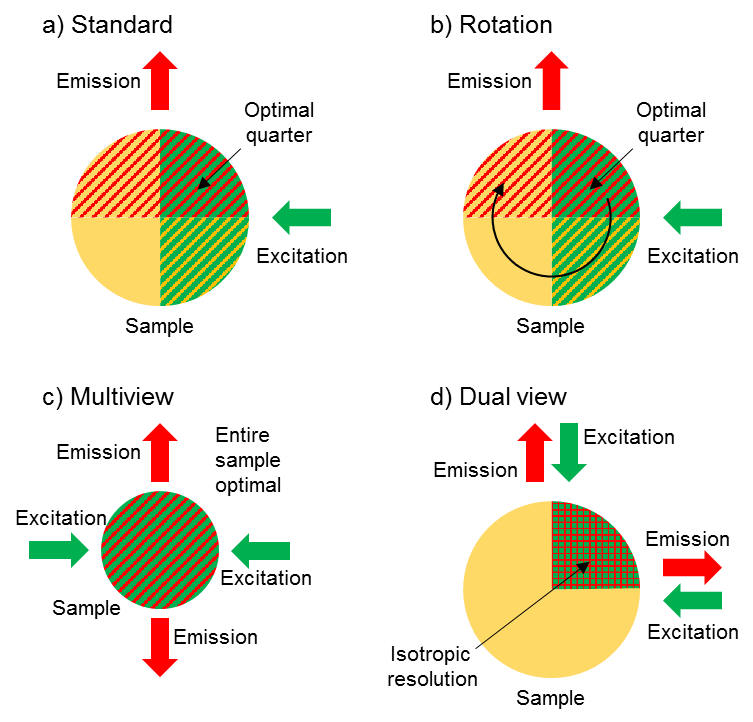
\includegraphics[width=\columnwidth]{spim_optimal_imaging.png}
	\caption{
	(a): The simple SPIM field of view – only a quarter of a sample has optimum illumination (green) and excitation (red).
	(b): by rotating a sample field of view can be quadrupled but at a cost in acquisition time. (c): By adding extra excitation and detection path the entire sample can be imaged without a rotation.
	(d): by making optical paths of a LSFM dual purpose a quadrant of a sample can be imaged from two orthogonal perspective and with correct image fusion achieve isotropic resolution.
	tod}
	\label{spim_optimal_imaging}
\end{figure}

\subsubsection{Optimal Orientation}

In a bid to maximise sample accessibility and numerical aperture, Betzig~\emph{et~al.}~\cite{chen_lattice_2014} commissioned a high NA (0.6) custom excitation objective to fit with their high NA (1.1) detection objective (Nikon CFI75).
In mounting the orthogonal pair at an angle such that they were flush so a flat surface, Betzig~\emph{et~al.} created the most unhindered sample mounting conditions realistically feasible using two objectives.
Tricks to circumvent objectives interfering with sample mounting are needed as high NA objectives are physically large.
%Numerical aperture depends on the $\sin$ of the collecting angle of light , intuitively this requires that the detecting objective to awkward in non-epifluorescence orientations. \todo{reword}
%Moreover, the desire for high resolution images can cause spacial incompatibility between both objectives.
Moreover,  high NA objectives typically have short working distances and require both objectives to be close, and likely cause spacial incompatibilities even with the narrowest excitation objectives.
See figure~\ref{fig:objectivecompatibility} for a detailed comparison.

\begin{figure}
	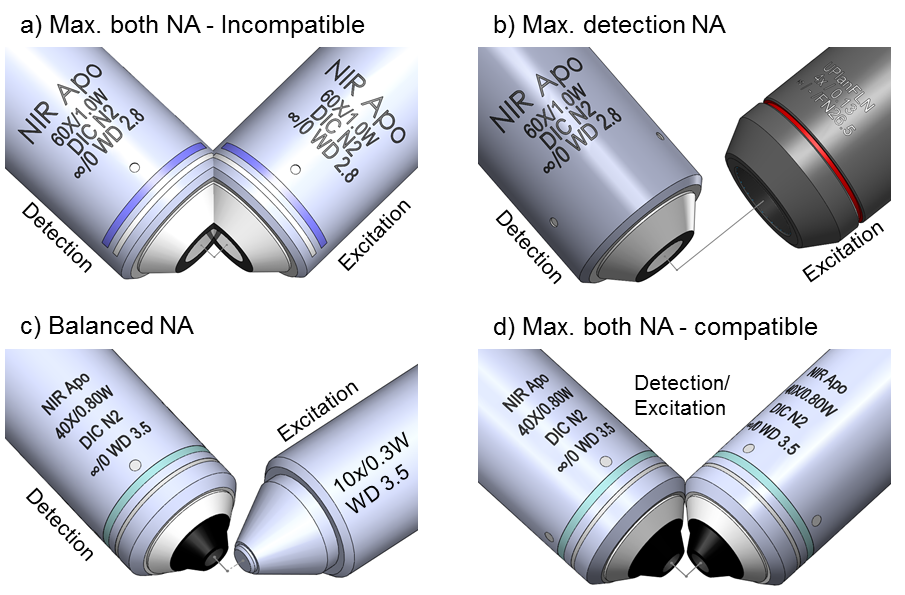
\includegraphics[width=\columnwidth]{objectivecompatibility}
	\label{fig:objectivecompatibility}
	\caption{}
\end{figure}

%Gaussian light sheet systems do not typically require such large NA excitation objectives meaning there are standard excitation objectives available.
%High NA objectives tend to have limited working distance and, in the orthogonal arrangements required for LSFM, have to be positioned very close to each other.

%suitably narrow such that flat substrates could be imaged.
%lattice light sheet style custom excitation.

%Gaussian beams don't need high NA excitation optics
%Large NA detection objectives have large collecting angles so a long working distance objective in desirable.


%subsection{MultiView}
\subsection{Multi-View}%\cite{swoger_multi-view_2007}

Shroff~\emph{et~al} introduced alternately imaging between each objective of the iSPIM in the form of the diSPIM~\cite{kumar_dual-view_2014}. %TODO Repeating myself
\footnote{This system is now a commercial light sheet solution provided by ASI.}
Axial resolution that would otherwise be lost to thick light sheets is recovered by switching the imaging and detection arms.
The two data sets captured by each camera are fused in post processing to provide near isotropic three dimensional resolution.
%\subsubsection{DualView}
%Shroff~\emph{et~al} not only pioneered the inverted SPIM (iSPIM) concept but also introduced alternately imaging between each objective in the form of diSPIM~\cite{kumar_dual-view_2014}. %TODO Repeating myself
%Axial resolution that would otherwise be lost to thick light sheets is recovered by switching the imaging and detection arms.
%The two data sets captured by each camera are fused in post processing.
%subsection{MuVU}
Where LSFM provides the most improvement over other techniques, such as in large, thick biological samples
%Where LSFM provides most improvement over other techniques
, scattering becomes significant both for excitation and emission light.
diSPIM however does not address inherent issues of scattering in thick samples, there is an \emph{optimal quarter} (see Figure~\ref{spim_optimal_imaging}) wherein excitation and emission photons are the least scattered.

Krzic~\emph{et~al} returned to the horizontal orientation of Huisken's SPIM, and chose their objectives wisely in MuVU-SPIM where two excitation and two detection objectives were packed around a hanging sample. %cite objectives (Krzic et al. 2012)
MuVu can reach all regions of its sample, but it cannot dodge scattering limitations homogeneously.
%\subsection{Tomography}
To minimise gross scattering, sample rotation is necessary, of course acquiring volumes tomographically raises its own unique issues such as volume registration, rotational synchonisation and lengthy acquisition times.
Regardless, for large samples two objectives in Huiksen's original SPIM provide a cost effective robust volumetric imaging solution; with projects like the OpenSPIM have received significant acceptance and community attention.

\section{Single Objective Light Sheet Microscopy}

\begin{itemize}
	\item[\checked] Axial Plane \cite{li_axial_2014}
	\item[\checked] Oblique Plane \cite{dunsby_optically_2008}
	\item[\checked] Fibre SPIM \cite{ploschner_multimode_2015}
	\item[\checked] Mirrored Cuvette,
	\item[\checked] Confocal adaptor
\end{itemize}

Prior to refinements in objective positioning Dunsby conceptualised a system for single objective light sheet microscopy.
The advent of such systems could provide a plug-and-play light sheet experience on commercial microscope frames.
Dunsby proposed illuminating the sample using a high NA objective whereby the light sheet would illuminate at an oblique angle to the optical axis, the detected signal is then retrieved using the same objective~\cite{dunsby_optically_2008}.
Optically the sample is conjugated to a virtual position where a pair of objectives (excitation and detection) analyse the virtual sample in a conventional light sheet manner.
The technique suffers from optical technology, only when using a high NA objective can the system fully capture detection perpendicular to excitation.
Unfortunately, OPM is an involved technique as it requires that a standard light sheet microscope is constructed behind a further optical relay system.

Virtual sample manipulation is alluring as one can perform virtual manipulations that in are physically impossible.
Zhang et al~\cite{li_axial_2014} created their virtual sample using a similar relay system to Dunksby\emph{et~al}, but crucially they positioned an atomically flat mirror which precisely rotated their virtual sample by $90^o$.
In doing so they could illuminate the real sample along the optical axis and their virtual projection from the mirror was imaged directly onto a camera using a standard wide field configuration.

Using small mirrors near the sample is another viable, though more restrictive, approach to single objective LSFM.\@
Galland~\emph{et~al.} fabricated  micro-wells with $45^o$ micro-mirrors~\cite{galland_3d_2015}, converting any commercial scanning microscope into a light sheet microscope.
Leica produce a similar solution in the form of an objective adapter which holds two mirrored surfaces near the sample creating a similar effect.
Both techniques limit the size of the sample and their sectioning capability heavily depends on the quality of the mirrors used.

Ploschneret al.~attempted to minimise the size of the second objective rather than remove it.
By substituting the second objective for a multimode fibre~\cite{ploschner_multimode_2015} not only could they provide more access to their samples, but they could also embed their excitation source into their imaging chamber.
Assuming that a multi-mode fibre operates deterministically on an input light source, they were able to correct for the fibre using an SLM and further demonstrated the system's ability to produce exotic beam profiles.

%TODO cite scape

%subsection{Axial Plane}~\cite{li_axial_2014}
%subsection{Oblique Plane}~\cite{dunsby_optically_2008}
%subsection{Fibre SPIM}~\cite{ploschner_multimode_2015}

%Optical fibre transforms input light, can comepnsate and produce light sheets, bessel light sheets and lattice etc. Demonstrated in 0.25 NA fibre. Could use soft glass fibre to prove concept further.

%subsection{Confocal adaptor}

% High NA objectives require short working distances and large apetures
% An asymmetric pair
% an NA of 0.3 is needed to create a micron thick miaskla kzas
% Gaussian beam illumination requires low NA excitation and so assymetric pairs are ideal with a high NA detection being then possible (with a loss of axial resolution)
% Bessel illumination however requires high NA to construct the thin buy extended sheets and so are commcercially infeasible. Betzig et al. notabley used a custom excitation objective.
% Biological samples should be given room.

% Hence the ‘vertical at 90o’ approach can very attractive even if it cannot boast high NA excitation.  Another limitation arises from geometrical compatibility of the objectives i.e. their opening angles cannot exceed 90o and the front lens radius of one objective should not exceed the working distance of the other objective.

%High NA detection and low NA excitation leads to high lateral resolution and low axial resolution.

\section{Illumination}

%\begin{itemize}
%	\item Variable Gaussian $\box$
%	\item Bessel\cite{gao_3d_2014}
%	\item Lattice light sheet.\cite{chen_lattice_2014}
%	\item Airy Beam $\box$
%	\item Multi-photon \checkmark~\cite{truong_deep_2011}
				%Comparison of Cost and Complexity?
%\end{itemize}

\subsection{Gaussian Techniques}
Illumination techniques have been proposed in a bid to circumvent the ubiquitous Gaussian beam extension versus thickness trade-off.
The most intuitive approach is accepting the loss of FOV produced by Gaussian illumination and moving the focus of this strip of high axial resolution light to different parts of the sample.
A final image can then be fused to achieve maximum axial resolution though with a direct cost for time of acquisition and photobleaching versus axial resolution, with an exceptionally high NA light sheet tending to becoming as slow and damaging as a confocal system . \todo[inline]{CITE Variable light-sheet.}
Fu~\emph{et~al.} proposed tiling multiple thin Gaussian light-sheets that are focally offset to create a similar tiling effect without the temporal loss~\cite{fu_imaging_2016}.
%The technique of tiled light-sheets was proposed recently whereby multiple thin Gaussian light-sheets are superimposed and focally offset to create a similar tiling effect without the temporal loss \cite{fu_imaging_2016}.
This effect was produced by using a Spatial Light Modulator whose hologram had superposed lens-like phase patterns superimposed.
This technique again suffers from the additional photo-dosage imparted by the undesirable lobes of the Gaussian beam, moreover these low resolution sections also contribute to fluorescent background reducing the net SNR of the system.
\subsection{Exotic Beams}
Species of exotic beam do exist which do not subscribe to classical Gaussian beam limitations.
%Airy beams, for instance, are non-diffracting, self healing beams.
% and I don't know anything about them over that Nikon use them?
Bessel beams are non-diffracting and self healing, meaning they reconstruct behind occlusions making them very desirable for light-sheet applications.
They can be optically constructed from either an axicon lens or a amplitude mask with a annual ring opening, the latter being inexpensive but the most optically lossy.
Unlike Gaussian optics their extension and thickness can be theoretically entirely decoupled, in practice a Bessel-Gauss beam only behaves over short distances \cite{gao_3d_2014} of up to $\sim 30\mu m$.
%\todo[inline]{how short?}
% with the thickness being controlled by the outter-most radius and their extension
%Be beams both self heal,
Bessel beams however suffer from having multiple undesirable orders, the more ideal a Bessel beam is the more intensity is retained in its outer rings.
As such a singular scanned Bessel beam itself causes a significant background.
Betzig~\emph{et~al.}\cite{chen_lattice_2014} exploited these additional orders, they constructed multiple Bessel beams in the scanning plane by superimposing a sinusoidal amplitude pattern on to an annular amplitude mask.
In doing so their undesirable orders constructed to reinforce the zeroth orders of the parallel beams.
Finally they adjusted their now lattice light-sheet such that the outer orders above and below the scanning plane lay at minima in the detection point spread function reducing the net fluorescent axial background.
\subsubsection{Airy Beams}
Airy beams also self-heal similarly to Bessel beams but comparatively are more extended.
They are constructed using a coma-like phase pattern and exhibit characteristic a beam curvature.
Though they extend several fold further than Bessel beams, their curvature produces an asymmetric profile along the detection axis.
This is then required to be deconvolved in post processing.
Vettenburg~\emph{et~al}\cite{vettenburg_light-sheet_2014} demonstrated similar axial resolution improvement to Bessel beams whilst achieving a $\sim 3$ increase in field of view.
%It logically follows to create a lattice of Airy beams, this
%\todo[inline]{TODO cite.}
%Airy beams are generated with a phase distribution resembling coma aberrations. These beams are characterised by longer extent compared to typically achievable Bessel beams (e.g. extension of 160 µm versus 60 µm for a Bessel beam with similar diameter) (Vettenburg et al. 2014). However, the Airy beams exhibit a curvature similar to coma aberrations and unsymmetrical higher orders in the beam radial profile, creating a PSF with characteristic unsymmetrical elongation along the detection axis (Morris et al. 2009). These can be corrected by deconvolving a measured stack using software methods. This can produce better resolution images with larger field of view compared to similarly deconvolved images obtained using Gaussian and Bessel beams (Vettenburg et al. 2014). However, this superiority over Bessel beams has only been demonstrated in comparison with the most basic Bessel beam setup, which does not compensate for higher orders of the Bessel beam distribution

\begin{figure*}
	\centering
	\label{fig:scatteringandshadowing}
	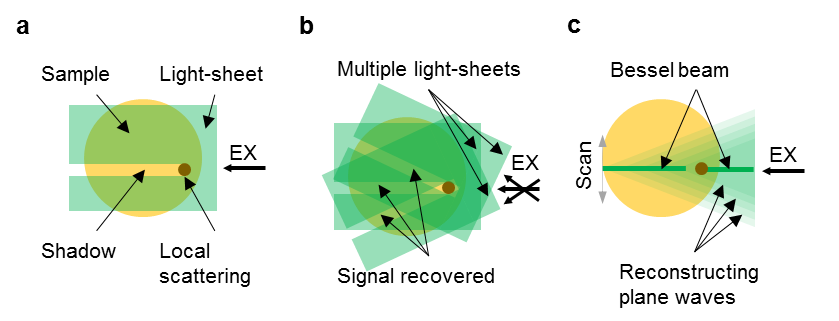
\includegraphics[width=\textwidth]{scatteringinlsfm}
\end{figure*}
\subsection{Thinner Beams}

Attempts to quantum mechanically narrow Gaussian Light sheets include using stimulated emission depletion and two photon emission (2P).
Using an addition laser to deplete, through stimulated emission (STED), out of plane fluorescence can narrow a Gaussian light sheet to $<1 \mu m$ \cite{friedrich_sted-spim:_2011}.
Two photon light sheet microscopy requires an excitation from two concomitant photons of cumulative energy sufficient bridge the required energy gap.
This requirement ensures that such excitation events are sufficiently rare and only occur where photon density is high.
%This requirement drastically reduces
%narrows the region in which fluorophores are likely to excite.
%By that two photons of cumulative energy sufficient to bridge the required energy gap, .
%By requiring that a fluorescent excitation only occurs when two photons of wavelength double that of the required energy gap,
In epi-fluorescent microscopes this occurs in the focal plane with the probability reducing quadratically along the imaging axis.
In light sheet microscopes this occurs at the axial centre of the light sheet making it much thinner than a comparable 1P excitation sheet.

%Exciting a

%%!TEX root = ../thesis.tex
%!TEX enableSynctex = true
%*******************************************************************************
%****************************** Third Chapter **********************************
%*******************************************************************************
% **************************** Define Graphics Path **************************
\ifpdf
    \graphicspath{{Chapter5/Figs/Raster/}{Chapter5/Figs/PDF/}{Chapter5/Figs/}}
\else
    \graphicspath{{Chapter5/Figs/Vector/}{Chapter5/Figs/}}
\fi

\chapter{Diffraction Limited Single Particle Tracking in SPIM}
\section{Single Particle Tracking}
\subsection{Applications}
\subsection{Techniques}
\section{Astigmatic Tracking}
\subsection{Template matching}
\subsubsection{Covariance}
\subsubsection{Cross correlation}
\subsection{Fitting} %Guassian fitting
\subsection{Neural Networks}
\section{Results}
\section{Virion Tracking using SPT}

%%!TEX root = ../thesis.tex
%!TEX enableSynctex = true
%*******************************************************************************
%****************************** Third Chapter **********************************
%*******************************************************************************
% **************************** Define Graphics Path **************************
\ifpdf
    \graphicspath{{Chapter6/Figs/Raster/}{Chapter6/Figs/PDF/}{Chapter6/Figs/}}
\else
    \graphicspath{{Chapter6/Figs/Vector/}{Chapter6/Figs/}}
\fi

\chapter{Biological sample mounting using Open Hardware}
\section{Long term embryo imaging}
\section{Live cell imaging}
\section{3D printed chamber}
\subsection{Design considerations}

%%!TEX root = ../thesis.tex
%!TEX enableSynctex = true
%*******************************************************************************
%****************************** Third Chapter **********************************
%*******************************************************************************
% **************************** Define Graphics Path **************************
\ifpdf
    \graphicspath{{Chapter7/Figs/Raster/}{Chapter7/Figs/PDF/}{Chapter7/Figs/}}
\else
    \graphicspath{{Chapter7/Figs/Vector/}{Chapter7/Figs/}}
\fi

\chapter{Faster confocal slit scanning light-sheet microscopy}
\section{Principles}
\section{Implementation}
\subsection{Slit-descanning} %Huisken did this in hyperspectral paper
\subsection{Improvement} %Could use fran's results or repeat mine (rather latter)
\subsection{Limitations} %Show that mismatch between beam and slit xy is bad and z is bad
\section{Double speed slit-scanning microscopy}
\subsection{Implementation} % Talk about SLM options
\subsubsection{Spatial light modulator} %Image of two beams with optimisation of intensity
\subsubsection{All optical solution} %Polarisation insensitive better etc, option to make bessel.
\subsection{Result}
\subsection{Summary)




% ********************************** Back Matter *******************************
% Backmatter should be commented out, if you are using appendices after References
%\backmatter 

% ********************************** Bibliography ******************************
\begin{spacing}{0.9}

% To use the conventional natbib style referencing
% Bibliography style previews: http://nodonn.tipido.net/bibstyle.php

\bibliographystyle{apalike}
%\bibliographystyle{plainnat} % use this to have URLs listed in References
\cleardoublepage
\bibliography{References/references} % Path to your References.bib file


% If you would like to use BibLaTeX for your references, pass `custombib' as 
% an option in the document class. The location of 'reference.bib' should be 
% specified in the preamble.tex file in the custombib section. 
% Comment out the lines related to natbib above and uncomment the following line.

% \printbibliography[heading=bibintoc, title={References}]


\end{spacing}

% ********************************** Appendices ********************************

\begin{appendices} % Using appendices environment for more functunality

% ******************************* Thesis Appendix A ****************************
\chapter{How to install \LaTeX} 

\section*{Windows OS}

\subsection*{TeXLive package - full version}
\begin{enumerate}
\item	Download the TeXLive ISO (2.2GB) from\\
\href{https://www.tug.org/texlive/}{https://www.tug.org/texlive/}
\item	Download WinCDEmu (if you don't have a virtual drive) from \\
\href{http://wincdemu.sysprogs.org/download/}
{http://wincdemu.sysprogs.org/download/}
\item	To install Windows CD Emulator follow the instructions at\\
\href{http://wincdemu.sysprogs.org/tutorials/install/}
{http://wincdemu.sysprogs.org/tutorials/install/}
\item	Right click the iso and mount it using the WinCDEmu as shown in \\
\href{http://wincdemu.sysprogs.org/tutorials/mount/}{
http://wincdemu.sysprogs.org/tutorials/mount/}
\item	Open your virtual drive and run setup.pl
\end{enumerate}

or

\subsection*{Basic MikTeX - \TeX~ distribution}
\begin{enumerate}
\item	Download Basic-MiK\TeX (32bit or 64bit) from\\
\href{http://miktex.org/download}{http://miktex.org/download}
\item	Run the installer 
\item	To add a new package go to Start >> All Programs >> MikTex >> Maintenance (Admin) and choose Package Manager
\item	Select or search for packages to install
\end{enumerate}

\subsection*{TexStudio - \TeX~ editor}
\begin{enumerate}
\item	Download TexStudio from\\
\href{http://texstudio.sourceforge.net/\#downloads}
{http://texstudio.sourceforge.net/\#downloads} 
\item	Run the installer
\end{enumerate}

\section*{Mac OS X}
\subsection*{MacTeX - \TeX~ distribution}
\begin{enumerate}
\item	Download the file from\\
\href{https://www.tug.org/mactex/}{https://www.tug.org/mactex/}
\item	Extract and double click to run the installer. It does the entire configuration, sit back and relax.
\end{enumerate}

\subsection*{TexStudio - \TeX~ editor}
\begin{enumerate}
\item	Download TexStudio from\\
\href{http://texstudio.sourceforge.net/\#downloads}
{http://texstudio.sourceforge.net/\#downloads} 
\item	Extract and Start
\end{enumerate}


\section*{Unix/Linux}
\subsection*{TeXLive - \TeX~ distribution}
\subsubsection*{Getting the distribution:}
\begin{enumerate}
\item	TexLive can be downloaded from\\
\href{http://www.tug.org/texlive/acquire-netinstall.html}
{http://www.tug.org/texlive/acquire-netinstall.html}.
\item	TexLive is provided by most operating system you can use (rpm,apt-get or yum) to get TexLive distributions
\end{enumerate}

\subsubsection*{Installation}
\begin{enumerate}
\item	Mount the ISO file in the mnt directory
\begin{verbatim}
mount -t iso9660 -o ro,loop,noauto /your/texlive####.iso /mnt
\end{verbatim}

\item	Install wget on your OS (use rpm, apt-get or yum install)
\item	Run the installer script install-tl.
\begin{verbatim}
	cd /your/download/directory
	./install-tl
\end{verbatim}
\item	Enter command `i' for installation

\item	Post-Installation configuration:\\
\href{http://www.tug.org/texlive/doc/texlive-en/texlive-en.html\#x1-320003.4.1}
{http://www.tug.org/texlive/doc/texlive-en/texlive-en.html\#x1-320003.4.1} 
\item	Set the path for the directory of TexLive binaries in your .bashrc file
\end{enumerate}

\subsubsection*{For 32bit OS}
For Bourne-compatible shells such as bash, and using Intel x86 GNU/Linux and a default directory setup as an example, the file to edit might be \begin{verbatim}
edit $~/.bashrc file and add following lines
PATH=/usr/local/texlive/2011/bin/i386-linux:$PATH; 
export PATH 
MANPATH=/usr/local/texlive/2011/texmf/doc/man:$MANPATH;
export MANPATH 
INFOPATH=/usr/local/texlive/2011/texmf/doc/info:$INFOPATH;
export INFOPATH
\end{verbatim}
\subsubsection*{For 64bit OS}
\begin{verbatim}
edit $~/.bashrc file and add following lines
PATH=/usr/local/texlive/2011/bin/x86_64-linux:$PATH;
export PATH 
MANPATH=/usr/local/texlive/2011/texmf/doc/man:$MANPATH;
export MANPATH 
INFOPATH=/usr/local/texlive/2011/texmf/doc/info:$INFOPATH;
export INFOPATH

\end{verbatim}



%\subsection{Installing directly using Linux packages} 
\subsubsection*{Fedora/RedHat/CentOS:}
\begin{verbatim} 
sudo yum install texlive 
sudo yum install psutils 
\end{verbatim}


\subsubsection*{SUSE:}
\begin{verbatim}
sudo zypper install texlive
\end{verbatim}


\subsubsection*{Debian/Ubuntu:}
\begin{verbatim} 
sudo apt-get install texlive texlive-latex-extra 
sudo apt-get install psutils
\end{verbatim}

%!TEX root = ../thesis.tex
% ******************************* Thesis Appendix B ********************************


\end{appendices}

% *************************************** Index ********************************
\printthesisindex % If index is present

\end{document}
